\section{Lagrange Polynomial Interpolation}
\label{theory-lagrange}

Below we present the theory of interpolation using Lagrange Polynomials, applied to simplex geometries, This section is inspired by \textbf{[wiki-lagrange], [Papers]}, and is a summary of well-known results. The goal is to construct a mapping $\vec{x} = \vec{p}(\vec{r})$ from local coordinates of an entity to global coordinates of the domain. In its own local coordinates, the entity is called \citeDune{} a reference element. A simplex reference element is given by the following coordinates: \\

\noindent
\begin{tabular}{l l l}
\hline
  Label & Dimension & Coordinates \\ \hline
  $\Delta_0$ & 0 & $\{ \}$ \\
  $\Delta_1$ & 1 & $\{ 0\}, \{ 1\}$ \\
  $\Delta_2$ & 2 & $\{ 0, 0 \}, \{ 1, 0 \}, \{ 0, 1 \}$ \\
  $\Delta_3$ & 3 & $\{ 0, 0, 0 \}, \{ 1, 0, 0 \}, \{ 0, 1, 0 \}, \{ 0, 0, 1 \}$ \\
\end{tabular} \\

\noindent
Local simplex geometries can be parametrized using the local coordinate vector $\vec{r}$: \\

\noindent
\begin{tabular}{l l l}
\hline
  Entity      & Parametrization    & Range \\ \hline
  Edge        & $\vec{r}=(u)$      & $u \in [0,1]$ \\
  Triangle    & $\vec{r}=(u,v)$    & $u \in [0,1]$ and $v \in [0, 1-u]$ \\
  Tetrahedron & $\vec{r}=(u,v,w)$  & $u \in [0,1]$, $v \in [0, 1-u]$ and $w \in [0, 1-u-v]$ \\
\end{tabular} \\

\subsection{Interpolatory Vertices}
\label{theory-lagrange-vertices}

\noindent
In order to define the curvilinear geometry, a set of real geometry points $\vec{x}_i = \vec{p}_i(\vec{r}_i)$ is given to be interpolated over. By convention, the real geometry is sampled over a structured grid on a reference simplex, namely
\[\vec{r}_{i,j,k} = \frac{(i,j,k)}{Ord}, \;\;\; i=[0..Ord], \;\;\; j=[0..Ord-i], \;\;\; k=[0..Ord-i-j]\]
where $Ord$ is the interpolation order of the surface. Thus, points from this uniform grid in local coordinates must be mapped to the provided points in global coordinates. It is the job of the meshing software (e.g. GMSH\citeGMSH{}) to ensure that the global geometry of an entity is non-singular / non-self-intersecting. In principle, a non-uniform grid could be used in order to minimize the effect of Runge phenomenon \textbf{CITE\_RUNGE}, However, it is not an issue for lower dimensions. \\

\noindent
One can verify that the above discretization generates the following number of interpolatory points: \\

\noindent
\begin{tabular}{l l l l l l}
\hline
  Entity \textbackslash Order & 1 & 2  & 3  & 4  & 5 \\ \hline
  Edge                        & 2 & 3  & 4  & 5  & 6 \\
  Triangle                    & 3 & 6  & 10 & 15 & 21 \\
  Tetrahedron                 & 4 & 10 & 20 & 35 & 56 \\
\end{tabular} \\


\subsection{Interpolatory Polynomials}
\label{theory-lagrange-polynomials}

\noindent
The number of interpolatory points above exactly matches the total number of monomials necessary to construct a complete polynomial of order $Ord$ or less. It is quite obvious, since the above discretization matches the binomial/trinomial triangle. We define the functions $z^{(1,i)}(u)$, $z^{(2,i)}(u,v)$ and $z^{(3,i)}(u,v,w)$ as the set of all monomials of corresponding order, where the first parameter is dimension of the entity, and the 2nd is the polynomial order:
\begin{itemize}
	\item edge: \\
		$z^{(1,1)}(u) = \{1, u\}$, \\
		$z^{(1,2)}(u) = \{1, u, u^2\}$, \\
		$z^{(1,3)}(u) = \{1, u, u^2, u^3\}$, \\
		$z^{(1,4)}(u) = \{1, u, u^2, u^3, u^4\}$, \\
		$z^{(1,5)}(u) = \{1, u, u^2, u^3, u^4, u^5\}$, \\
		etc
	\item face:	\\
		$z^{(2,1)}(u,v)	= \{1, u, v\}$, \\
		$z^{(2,2)}(u,v) = \{1, u, v, u^2, uv, v^2\}$, \\
		etc
	\item tetrahedron: \\
		$z^{(2,1)}(u,v,w) = \{1, u, v, w\}$, \\ 
		$z^{(2,2)}(u,v,w) = \{1, u, v, w, u^2, uv, v^2, wu, wv, w^2\}$, \\
		etc
\end{itemize}

\noindent
Ultimately, we wish to approximate the mapping $\vec{p}(\vec{r})$ by a polynomial of the order $Ord$, such that it exactly fits the provided interpolatory vertices $\vec{x}_i$. Since there are as many interpolatory vertices as there are monomials, such a polynomial will be unique. This allows the simplex geometries to be interpolated by \textit{complete} basis of a given order. This is not the same for all entities. For example, for hexahedra, these numbers do not match, therefore one either has to use interpolation of incomplete polynomial order, or choose a more sophisticated local discretization. \textbf{[Volakis2010]} choose the first approach, interpolating a 9 node 2nd order rectangle with 4th order incomplete polynomial which has a convenient separable tensor product form. \\

\noindent
But back to simplices. One way to write such a polynomial approximation is
\begin{equation}
	\vec{p}(\vec{r}) = \sum_j L_j(\vec{r})\vec{p}_j 
\end{equation}
\noindent
where the Lagrange Polynomials $L_j$ are defined by their interpolatory property
\begin{equation}
	\label{equation-lagrangepol-interpolatory-property}
	L_j(\vec{r}_i) = \delta_{ij}
\end{equation}
\noindent
for all interpolatory points $\vec{r}_i$. The advantage of this formulation is that the Lagrange Polynomials are independent of the exact coordinates ($\vec{x}_i$), and thus can be pre-computed and reused for all entities of a given order. \\

\noindent
It remains to determine the exact form of Lagrange Polynomials. We would like to prove that the following equation holds:
\begin{equation}
	\label{equation-lagrangepol-basis-link}
	z_i(\vec{r}) = \sum_j L_j(\vec{r}) z_i (\vec{r}_j) 
\end{equation}
\noindent
where $z_i$ is a vector of monomials defined above. This equation should hold for all $z^{(\dim, Ord)}$, where $\dim = \{1,2,3\}$. For $\dim < 3$ where $z$ is defined for less than 3 parameters, simply ignore the extra parameters in $\vec{r}$. \\

\noindent
The proof is quite simple. Both LHS and RHS are polynomials of order at most $Ord$, which means that they have at most $N_{Ord}$ free parameters, and therefore, if we can show that the equation holds for $N_{Ord}$ different parameter sets, then it holds for all others as well. And indeed, \eqref{equation-lagrangepol-basis-link} holds for all $\vec{r} = \vec{r}_k$ because of \eqref{equation-lagrangepol-interpolatory-property}. \\

\noindent
Finally, we can write \eqref{equation-lagrangepol-basis-link} as a vector equation
\begin{equation}
	\vec{z} (\vec{r}) = V \vec{L} (\vec{r})
\end{equation}
\noindent
where $V_{ij} = z_i (\vec{r}_j)$, and find the Lagrange polynomials by inverting $V$, namely
\begin{equation}
	\vec{L} (\vec{r}) = V^{-1} \vec{z} (\vec{r})
\end{equation}

\noindent
It is important to understand that the resulting interpolated geometry in global coordinates is NOT exhaustively defined by the shape of its boundary, as the geometry inside the entity also undergoes this polynomial transformation.


\subsection{Implementation for Simplices}
\label{subsection-simplexgrid}

\noindent
In this section we discuss how to efficiently enumerate the simplex interpolatory points, and to construct the reference simplex grid. \\

\noindent
Let us place a set of points $\vec{\eta} \in Z^{\dim}$ over simplex $\Delta^{\dim}_{\mathrm{len}}$. This can be done trivially
by using 3 for loops and pushing vectors into a vector
\begin{itemize}
	\item $\Delta^{1}_n = \{(i)\}$, for $i = [1$ to $n]$
	\item $\Delta^{2}_n = \{(j,i)\}$, for $i = [1$ to $n]$, $j = [1$ to $n - i]$
	\item $\Delta^{3}_n = \{(k,j,i)\}$, for $i = [1$ to $n]$, $j = [1$ to $n - i]$, $k = [1$ to $n - i - j]$
\end{itemize}

\noindent
Then, each point $(\Delta^{d}_n)_i$ corresponds exactly to the power of $u,v,w$ in the expansion of $(1 + u + v + w)^n$, namely
\[ (1 + u)^n = \sum_{i=0}^n C^{(\Delta^{1}_n)_i}_n u^{(\Delta^{1}_n)_{i,1}} \]
\[ (1 + u + v)^n = \sum_{i=0}^n C^{(\Delta^{1}_n)_i}_n u^{(\Delta^{1}_n)_{i,1}} v^{(\Delta^{1}_n)_{i,2}} \]
\[ (1 + u + v + w)^n = \sum_{i=0}^n C^{(\Delta^{1}_n)_i}_n u^{(\Delta^{1}_n)_{i,1}} v^{(\Delta^{1}_n)_{i,2}} w^{(\Delta^{1}_n)_{i,3}} \]

\noindent
where $C^{i}_n, C^{i,j}_n$ and $C^{i,j,k}_n$ are the binomial, trinomial and quatranomial coefficients. The powers of the parameters given in this way are exactly the complete monomial basis for a polynomial of order up to and including $d$. \\

\noindent
Also, it is convenient to note that $(\Delta^{d}_n)_i / n$ is exactly the parametric coordinates of the interpolation points on a regular grid over simplex. 

\begin{figure}[hp]
    \centering
    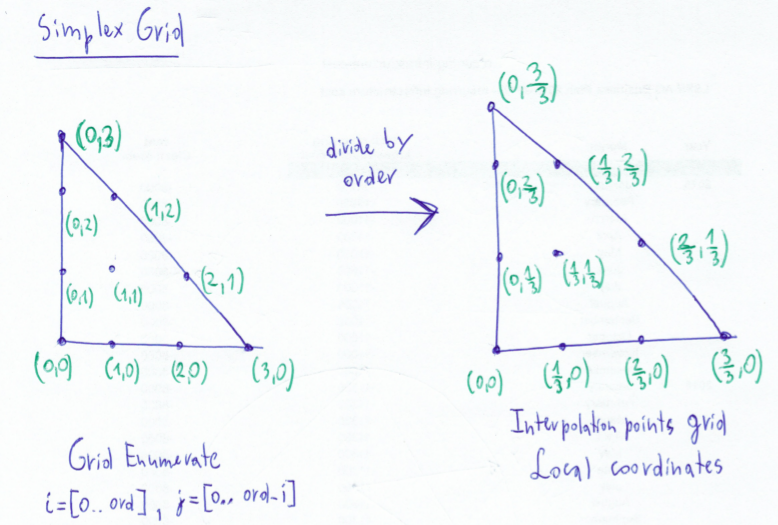
\includegraphics[scale=0.5]{doc-pics/pic-simplex-grid.png}
    %\caption{Awesome Image}
    %\label{fig:awesome_image}
\end{figure}

\noindent
After the monomials and the parametric interpolation points have been constructed, it remains to construct the interpolation matrix by evaluating the monomials at the interpolation points, then to invert the matrix, and multiply the monomial vector by it obtaining lagrange polynomials. This has been implemented both explicitly, by calculating all the lagrange interpolatory polynomials for simplices and writing them as functions, and implicitly, by introducing a polynomial class, which has all the above functionality, and thus generates a set of interpolatory polynomials which can be evaluated and integrated analytically by the code.